\chapter{State of the Art}\label{chap:sota}

%This chapter will be an overview of these types of approaches and technologies.

\section{Approaches to Creating Adaptable Software}\label{sec:approaches_to_creating_adaptable_software}

There are two main approaches to making systems adaptable: generative programming approaches and meta-architectures.

Generative programming methods approach the adaptability of a system by using an ontological model representative of this system to automatically create executable artifacts or code skeleton than can be further refined according to different needs.

Rails scaffolding and model generation is an excellent example of this approach, which will be further explained in Section \ref{sec:ror}.

On the other hand, systems created with a special architecture designed to adapt at runtime to new user requirements and rules by using descriptive information about the system model that can be interpreted at runtime are sometimes said to possess a ``reflective architecture'' or a ``meta-architecture''~\cite{YBJ01}.

\section{Software Product Lines}\label{sec:spl}

The Software Product Lines (SPL) software development paradigm is promoted as means of reducing time to market, increasing productivity, improving quality and gaining cost effectiveness and efficiency through large-scale reuse~\cite{TC06}. Software product line methods (SPLMs) are practices-based, or plan-driven, software development approaches in which a set of software-intensive systems that share a common, managed set of features are produced from a set of re-usable core assets in a predictive, rather than opportunistic way --- meaning artifacts are only created when the need for their use arises, instead of providing generic, reusable components.

\section{Domain-Driven Design}\label{sec:ddd}

Domain-Driven Design (henceforth referred to as DDD) is a philosophy and way of thinking, first described by Eric Evans in \cite{ddd_book}, aimed at accelerating software projects that have to deal with complicated domains,  with a two-fold premise \cite{ddd_website}:

\begin{itemize}
  \item For most software projects, the primary focus should be on the domain and domain logic; and
  \item Complex domain designs should be based on a model.
\end{itemize}

A third, informal premise is usually associated with DDD, wherein a collaboration between technical domain experts must exist, in order to quickly, over various iterations, reach the core of the problem's concept.

\section{Model-Driven Engineering}\label{sec:mda}

Model-Driven Engineering first appeared in 2001~\cite{Mil03} as an answer to the growing complexity system architectures. This growing complexity and the lack of a integrated view ``forced many developers to implement suboptimal solutions that unnecessarily duplicate code, violate key architectural principles, and complicate system evolution and quality assurance''~\cite{Sch06}.

To address these issues, Model-Driven engineering combines \emph{domain-specific modeling languages} (DSMLs) with \emph{transformation engines} and \emph{generators} in order to generate various types of artifacts, such as source code or alternative model definitions.

The usage of DSMLs ensures that the domain model is perfectly captured in terms of syntax and semantics. This guarantees a flatter learning curve as the concepts present in the language are already known by the domain experts. This also helps a broader range of experts, such as system engineers and experienced software architects, ensure that software systems meet user needs.

The ability to synthesize artifacts from models helps ensure the consistency between application implementations and analysis information associated with functional and quality of service requirements captured by models.

\section{Frameworks}\label{sec:frameworks}

Frameworks provide a series of loosely-coupled components created for a specific purpose that provide generic functionality for the creation of software systems. These components can be overridden or specialized in order to create specific functionality. Frameworks can improve developer productivity and improve the quality, reliability and robustness of new software.  Developer productivity is improved by allowing developers to focus on the unique requirements of their application instead of spending time on application infrastructure. XNA~\cite{xna} and RoR~\cite{rubyonrails} are good examples of popular frameworks that aim to cut development time and costs in very different scenarios.

Frameworks can also be used together with code-generation techniques~\cite{DH04, rails_generators} to improve the overall production speed and ease of use.

\section{Metaprogramming}\label{sec:metaprogramming}

As defined by Robert D. Cameron and M. Robert Ito in~\cite{CI84},

\begin{quote}
 ``A metaprogramming system is a programming facility (subprogramming system or language) whose basic data objects include the programs and program fragments of some particular programming language, known as the target language of the system. Such systems are designed to facilitate the writing of metaprograms, that is, programs about programs. Metaprograms take as input programs and fragments in the target language, perform various operations on them, and possibly, generate modified target-language programs as output.''
\end{quote}

To put it simply, metaprogramming is code that manipulates code. The advantages of this paradigm have been described many times in software reuse literature. The translation of high-level descriptions into low-level implementations (by means of application generators) allows a developer to focus on specification based on tested standards rather than implementation, making tasks like system maintenance and evolution much easier and affordable~\cite{Bas87, Cle88}. %However, the focus of these methodologies is directed to the code level rather than the underlying domain concepts.

\section{Aspect-Oriented Programming}\label{sec:aspect_oriented_programming}

Aspect-Oriented Programming is a programming paradigm that isolates secondary or auxiliary behaviours from the implementation of the main business logic. It has been proposed as a viable implementation of modular crosscutting concerns. Since crosscutting concerns cannot be properly modularized within object-oriented programming, they are expressed as aspects and are composed, or woven, with traditionally encapsulated functionality referred to as components~\cite{KM05, Ste06}. This paradigm has been gaining some momentum particularly because even conceptually simple crosscutting concerns such as tracing during debugging and synchronization, lead to tangling, in which code statements addressing the crosscutting concern become interlaced with those addressing other concerns within the application~\cite{LC03}.

Many AOP implementations work by automatically injecting new code into existing classes (a process which is commonly called \emph{decorating} a class), effectively adding new functionalities that promote extensive code reuse~\cite{Ste06, LC03, metaclass_programming_in_python}.

\section{Design Patterns}\label{sec:design_patterns}

As stated by the architect Christopher Alexander in \cite{christopher_alexander_a_pattern_language}:

\begin{quote}
  ``Each pattern describes a problem which occurs over and over again in our environment, and then describes the core of the solution to that problem, in such a way that you can use this solution a million times over, without ever doing it the same way twice''
\end{quote}

Despite applying the term \emph{design pattern} to architectural problems, it is possible to transpose these ideas to object-oriented design. As such, a design pattern is, to put it simply, a common solution to a recurring problem. \cite{gang_of_four} then defines the four essential components of a design pattern:

\begin{itemize}
  \item The \textbf{Name}, which captures the essence of a design pattern and describes it in as few words as possible (one or two, usually); \\
  \item The \textbf{Problem}, which describes the conditions necessary to apply the pattern, by explaining the problem and its context; \\
  \item The \textbf{Solution}, which describes the elements that make up the design, their relationships, responsibilities, and collaborations, while keeping it as general as possible, so that its application is possible within multiple contexts: \\
  \item The \textbf{Consequences}, which denotes the results and trade-offs pertaining to the application of the pattern, allowing the evaluation of alternative designs and understanding the costs and benefits of applying the pattern. \\
\end{itemize}

\section{Adaptive Object-Models}\label{sec:aom}

Despite all of the advances in the aforementioned areas, most (if not all) the currently used techniques and methodologies still require a programmer or a domain expert in order to modify a system definition and model. A specific type of architecture is required for the end-user to be able to modify part or the entirety of a system to fit the underlying model to their own needs.

As such, an end-user is not expected to have any kind of knowledge about programming, design patterns and system architectures, or about a system of this type comes to be. However, the end-user is sometimes the most knowledgeable part of the development chain, in regards to how the system should behave.

\subsection{AOM Architecture}\label{sec:aom_architecture}

An Adaptive Object-Model pattern is a system architecture that represents classes, attributes, relationships, and behavior as \emph{metadata}. The system definition is based on instances of model abstractions rather than classes. This allows the modification of these model abstractions in runtime to reflect changes in the domain, effectively modifying the system behavior. As a direct consequence, the system instantly reacts to these changes, making it adaptable to change, without the need for recompiling or redeploying~\cite{YBJ01}. This architectural pattern is akin to the Meta Object Facility (MOF), which main purpose is to provide a metadata management and implementation framework. The basic architecture is divided into four tiers, each one compliant with the higher level\cite{mof}, as depicted in Fig.~\ref{fig:aom_mof_levels}:

\begin{figure}[H]
  \centering
  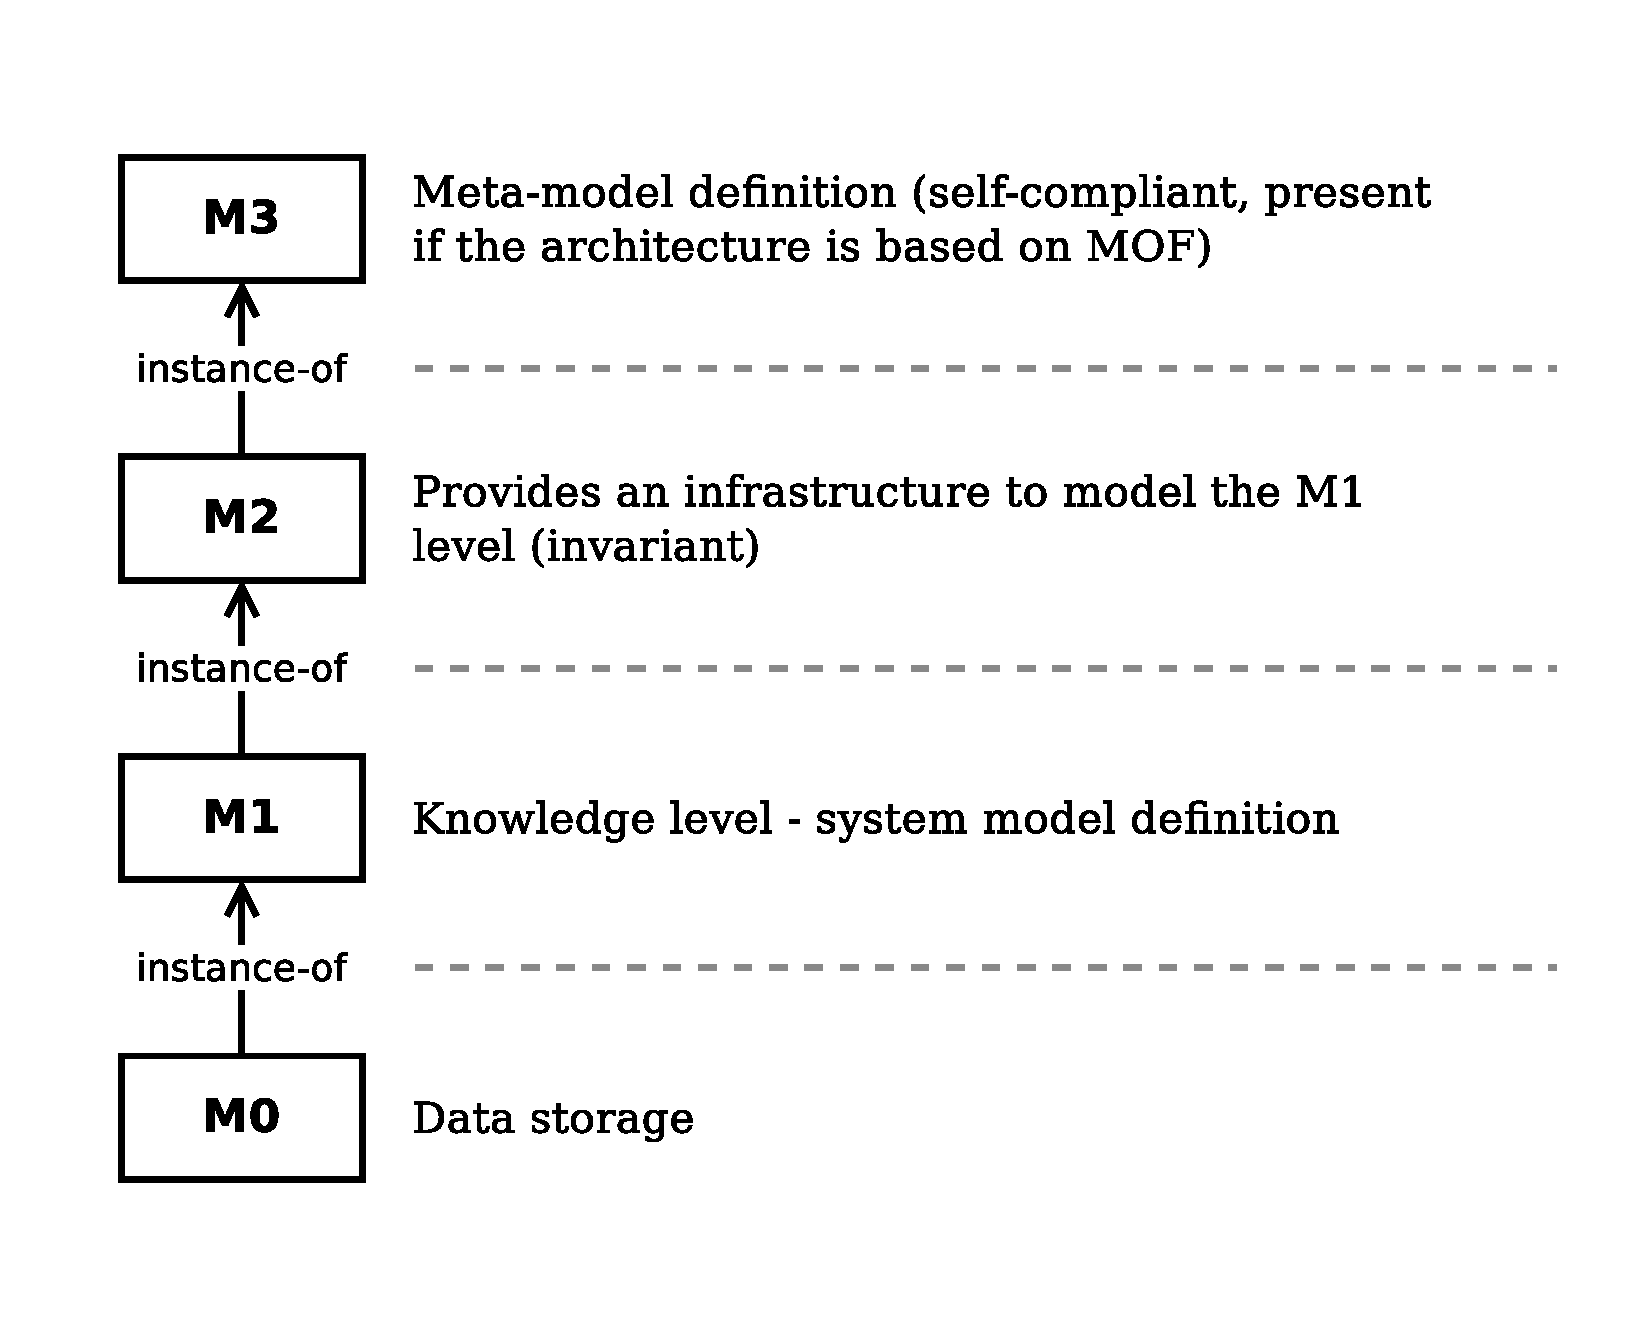
\includegraphics[width=120mm]{aom_mof_levels}
  \caption{MOF levels}
  \label{fig:aom_mof_levels}
\end{figure}

%\begin{itemize}
%  \item M0: Data storage
%  \item M1: Knowledge level --- system model definition
%  \item M2 (invariant): Meta-model --- provides an infrastructure to model the M1 level
%  \item M3 (invariant): Meta-model definition (self-compliant, present if the architecture is based on MOF)
%\end{itemize}

This kind of architecture relies on a series of design patterns: the \textsc{Type-Object} and \textsc{Property} patterns form the basic building blocks whereupon the AOM architecture settles. Despite being extremely simple, they create the fundamental infrastructure able to decouple the model definition from code-level implementation. In addition to these two patterns mentioned, other design patterns which are able to form an AOM architecture will be described, as well as the interactions between them.

\subsubsection{\textsc{Type-Object} Pattern}\label{sec:type-object_pattern}

Object-oriented languages usually structure a program as a set of classes that define the structure and behavior of objects, usually organizing them as a separate class for each object type, which means that any structural change to the model requires code-level modifications. However, variable systems are usually faced with the problem of having a class that will be subclassed by an arbitrary number of specializations. The key to solving this problem is to detach the object definition from the code level and instead define it using meta-data --- generalizing objects and describing their variation as parameters. \textsc{Type-Object} works by splitting a class in two\cite{YBJ01}: the meta-class for the object to be created --- EntityType, and an instance of that class --- Type. Fig. \ref{fig:type-object_pattern} shows the UML class diagram for this design pattern.

\begin{figure}[H]
  \centering
  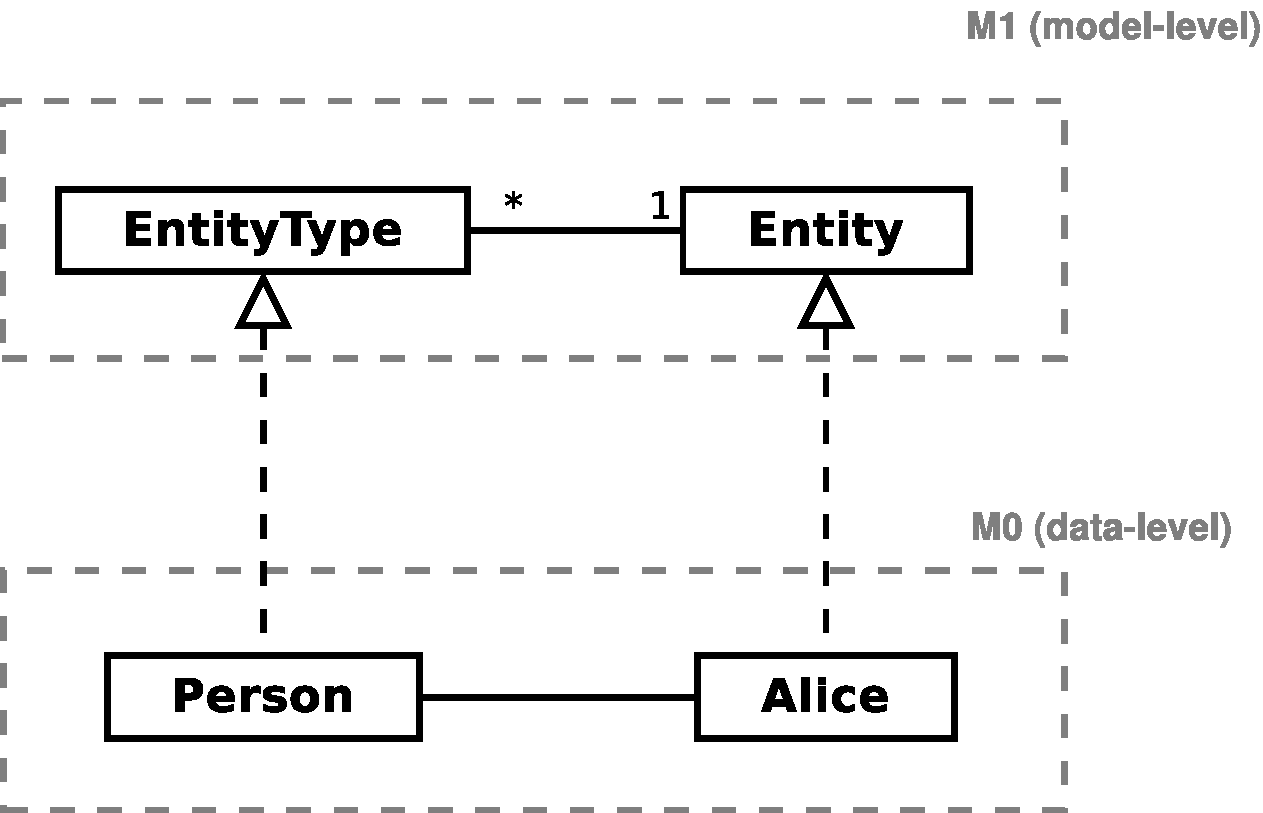
\includegraphics[width=75mm]{type_object.pdf}
  \caption{\textsc{Type-Object} pattern, adapted from \cite{metadata_and_active_object_models}}
  \label{fig:type-object_pattern}
\end{figure}

\subsubsection{\textsc{Property} Pattern}\label{sec:property_pattern}

Similar to the problem solved by the \textsc{Type-Object}, the \textsc{Property} pattern addresses the analogous issues of having the need to change the attributes (sometimes called \emph{members}) of a class. The anticipation of these structural changes leads to the \textsc{Property} pattern, where an attribute is split in two classes: the meta-class for the object to be created --- PropertyType, and an instance of that attribute --- Property. Fig. \ref{fig:property_pattern} represents the UML model for the \textsc{Property} design pattern.

\begin{figure}[H]
  \centering
  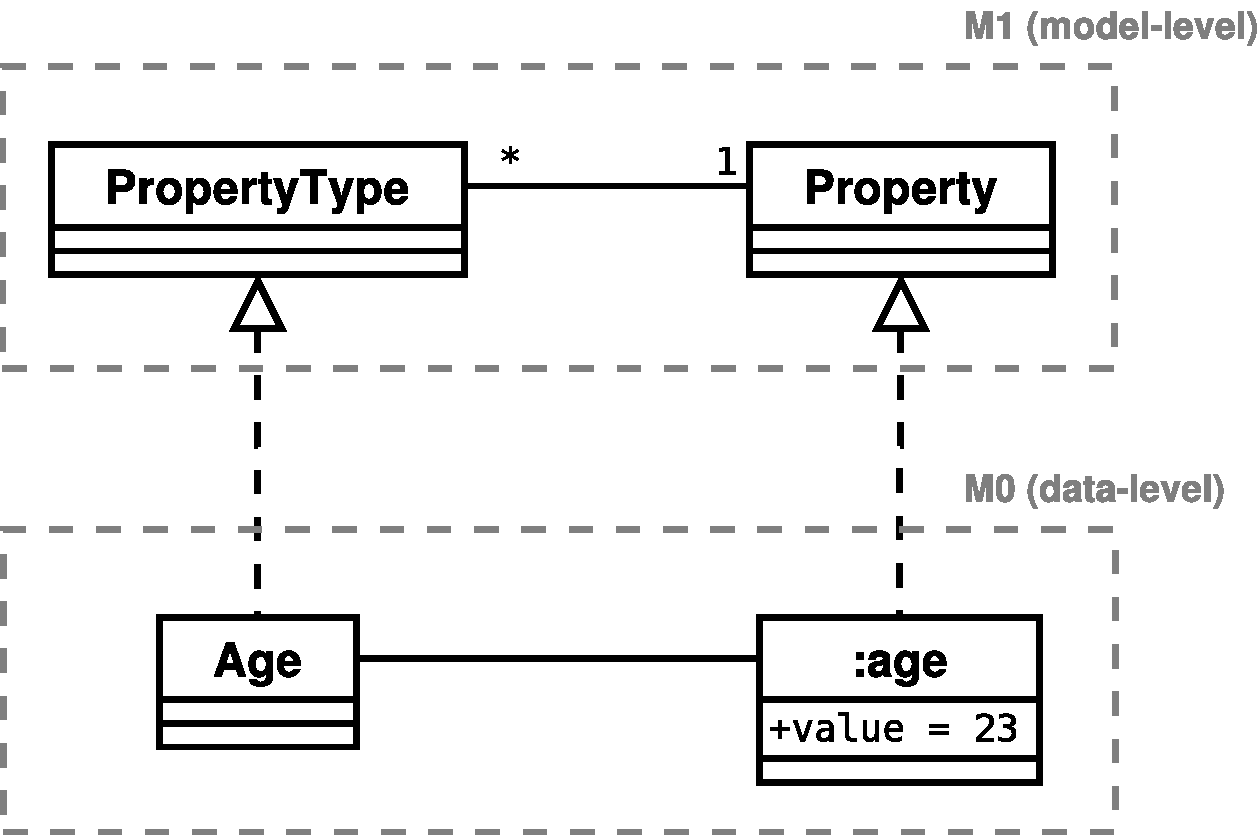
\includegraphics[width=80mm]{property}
  \caption{\textsc{Property} pattern, adapted from \cite{metadata_and_active_object_models}}
  \label{fig:property_pattern}
\end{figure}

\subsubsection{\textsc{Type-Square} Pattern}\label{sec:type-square_pattern}

Usually a class is modeled with a number of different attributes, representing their real world counterparts. So, in order to make a runtime modifiable class, an user must be able to modify both its \emph{definition} and \emph{attributes}. The answer to this issue is to use both \textsc{Type-Object} and \textsc{Property} patterns at the same time, creating what is known as the \textsc{Type-Square} pattern --- which forms the basis of any AOM architecture~\cite{YJ02}. Figure \ref{fig:type_square} shows the UML model for this pattern.

\begin{figure}[H]
  \centering
  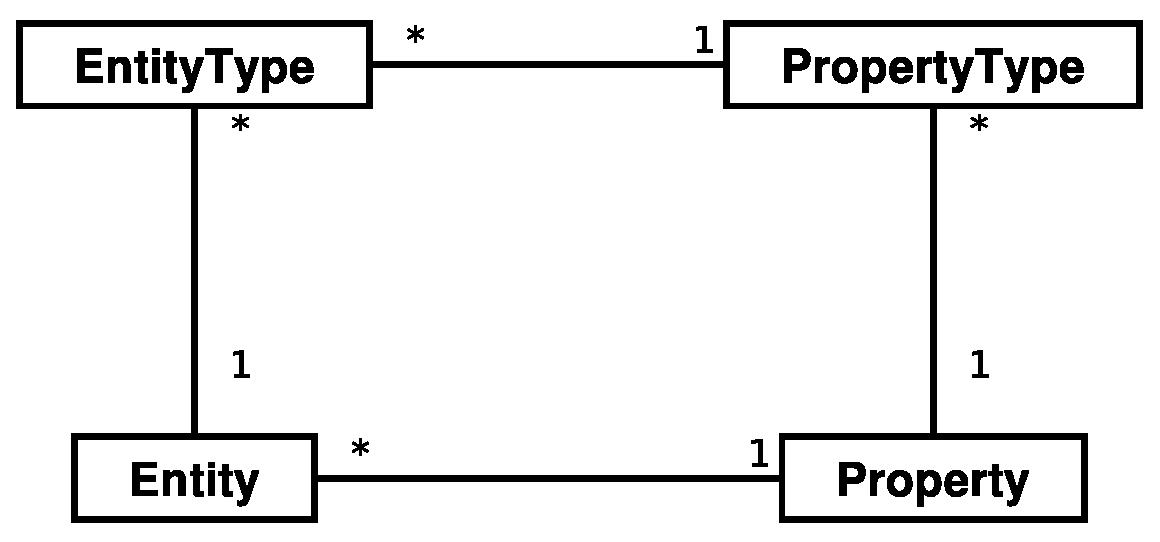
\includegraphics[width=90mm]{type_square}
  \caption{\textsc{Type-Square} pattern, adapted from \cite{YBJ01}}
  \label{fig:type_square}
\end{figure}

\subsubsection{\textsc{Strategy} and \textsc{Rule Object} Pattern}\label{sec:strategy_pattern}

The original goal of the \textsc{Strategy} pattern is to, given a set of algorithms, encapsulate each one in order to use them interchangeably which allows the easy usage of different strategies to solve different problems\cite{gang_of_four}.

As AOM architectures are concerned, this pattern is used to perform user-defined validations for user input, whichever they may be. An example can be found on Fig.~\ref{fig:strategy_pattern}.

\begin{figure}[H]
  \centering
  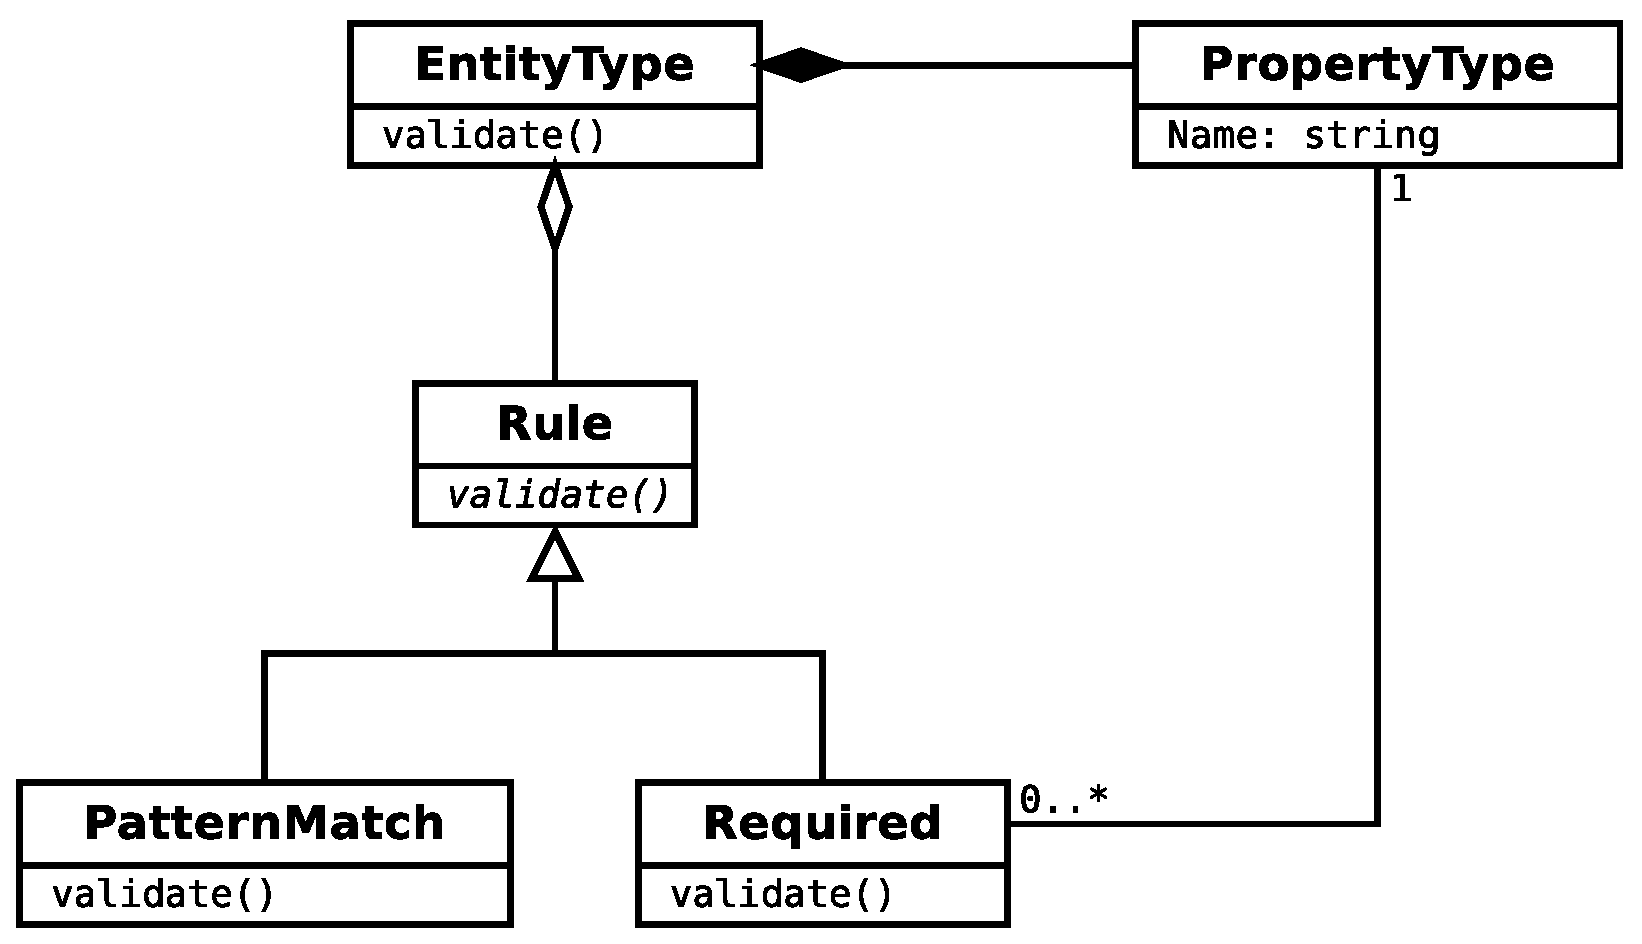
\includegraphics[width=130mm]{strategy}
  \caption{\textsc{Strategy} pattern, as applied to an AOM architecture, adapted from \cite{gang_of_four}}
  \label{fig:strategy_pattern}
\end{figure}

\subsubsection{\textsc{Interpreter} Pattern}\label{sec:interpreter_pattern}

The \textsc{Interpreter} pattern commonly is used when a recurring problem within a platform arises. When this is the case, it might be fruitful to define a simple language to solve these types of problems \cite{gang_of_four}. Regarding AOMs, this pattern, coupled with \textsc{Strategy} (described in \ref{sec:strategy_pattern}), is used to allow users to express complex restrictions on the values of properties present in the system. Fig.~\ref{fig:interpreter_pattern} shows how this pattern is usually applied to AOM architectures, as described in \cite{phd_hugo_ferreira}.

\begin{figure}[H]
  \centering
  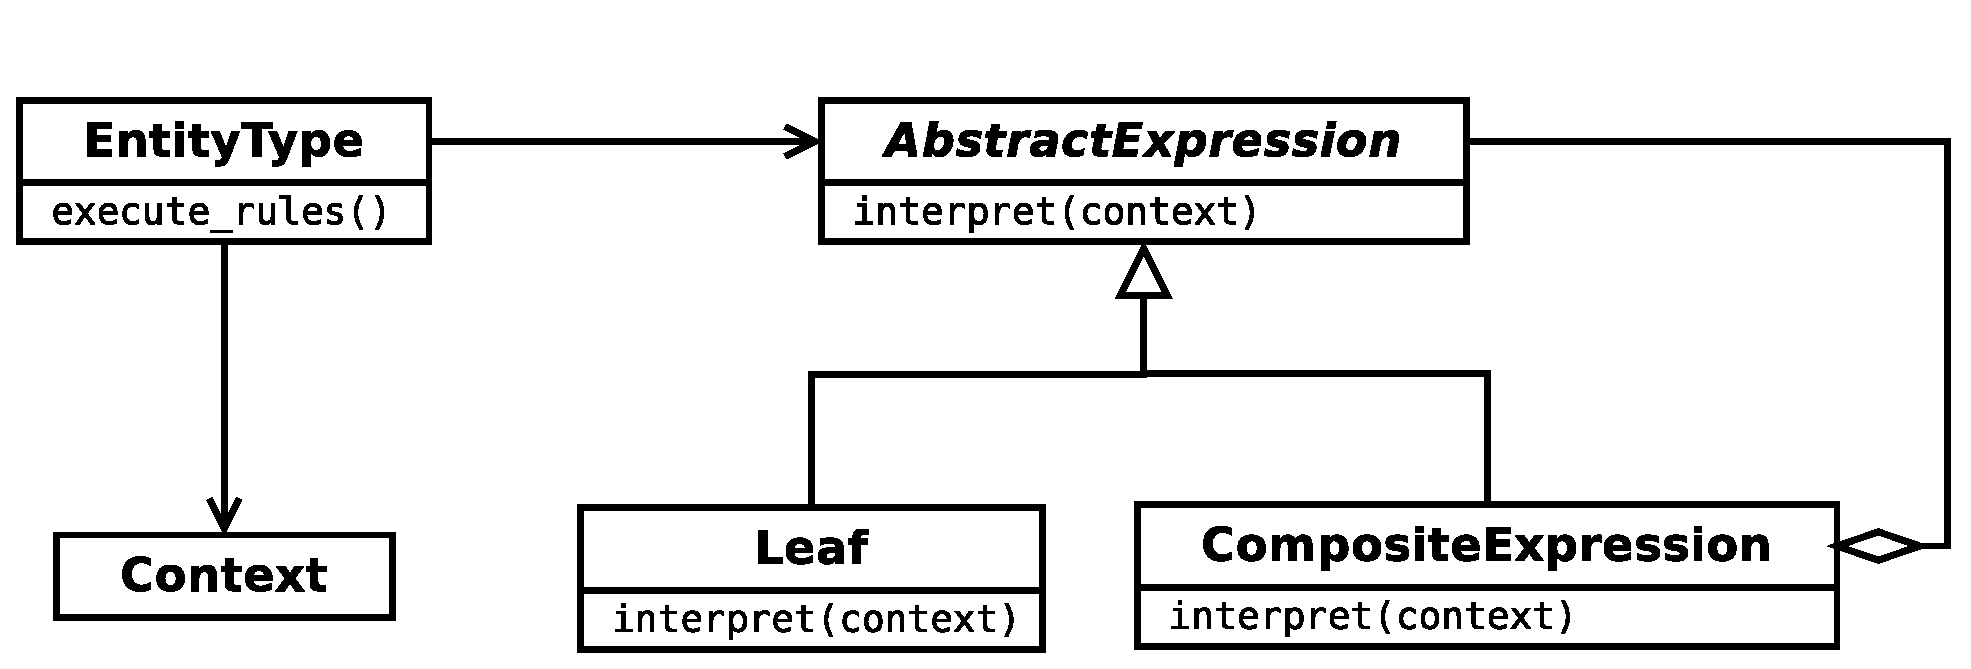
\includegraphics[width=140mm]{interpreter}
  \caption{\textsc{Interpreter} pattern, as applied to an AOM architecture, adapted from \cite{gang_of_four}}
  \label{fig:interpreter_pattern}
\end{figure}

\subsubsection{\textsc{System Memento} Pattern}\label{sec:system_memento_pattern}

The \textsc{System Memento} Pattern is used when one wishes to preserve the different states a system has achieved upon its evolution. The usage of this pattern allows the decoupling of the state from the objects themselves and promotes reusability as the same versioning mechanism can be applied to any entity present in the system. This pattern usually states that an entity in a system (henceforth referred to as a \emph{Thing}) is a composition of \emph{States} (as shown on Fig.~\ref{fig:system_memento}), which, when timestamped, work as evolutionary line for each of the \emph{Things} it is related with. Finally, a \emph{Version} is a collection of all of the \emph{States} in a system, effectively creating a snapshot of the whole system at a given point in time.

\begin{figure}[H]
  \centering
  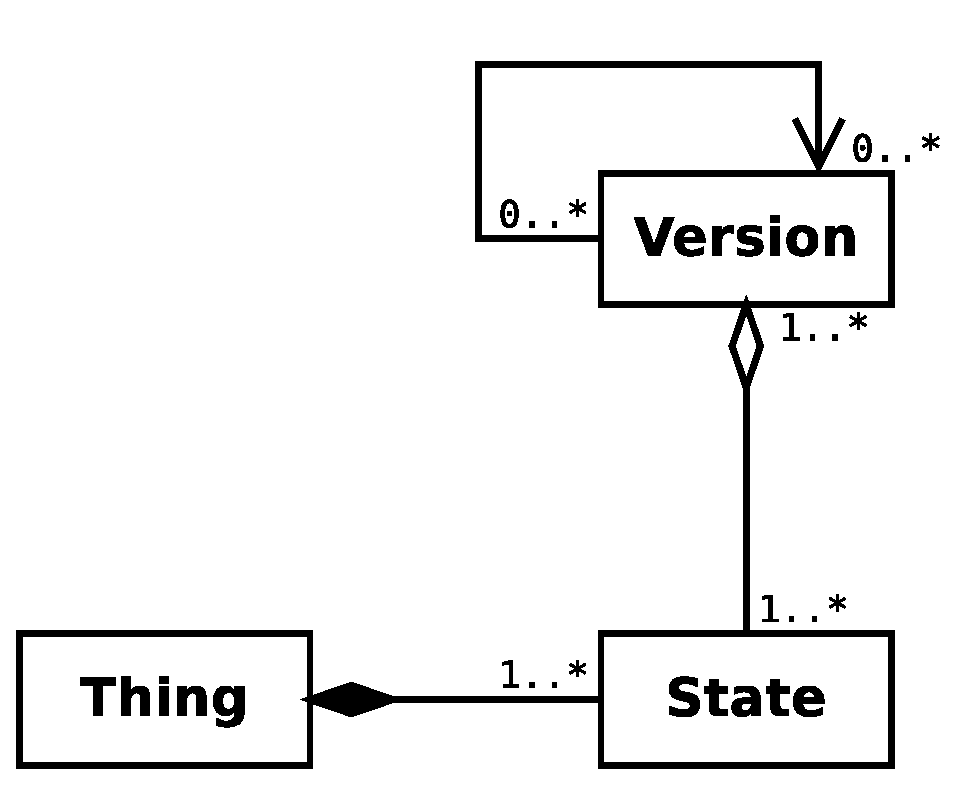
\includegraphics[width=70mm]{system_memento}
  \caption{\textsc{System Memento} pattern, adapted from \cite{patterns_data_and_metadata_evolution_in_aoms}}
  \label{fig:system_memento}
\end{figure}

\subsubsection{Relationships Between Entities}\label{sec:relationships_between_entities}

Yoder \textit{et al.}\cite{YJ02} describes the relationships between AOM classes by using the \textsc{Accountability} pattern~\cite{fowler, hay}. The \textsc{Accountability} pattern is used when there is a need to express multiple types of relationships between \emph{parties} (regardless of what their types may be), all of which carry a different meaning\cite{fowler_accountability}. This pattern is shown on Figure~\ref{fig:accountability}.

\begin{figure}[H]
  \centering
  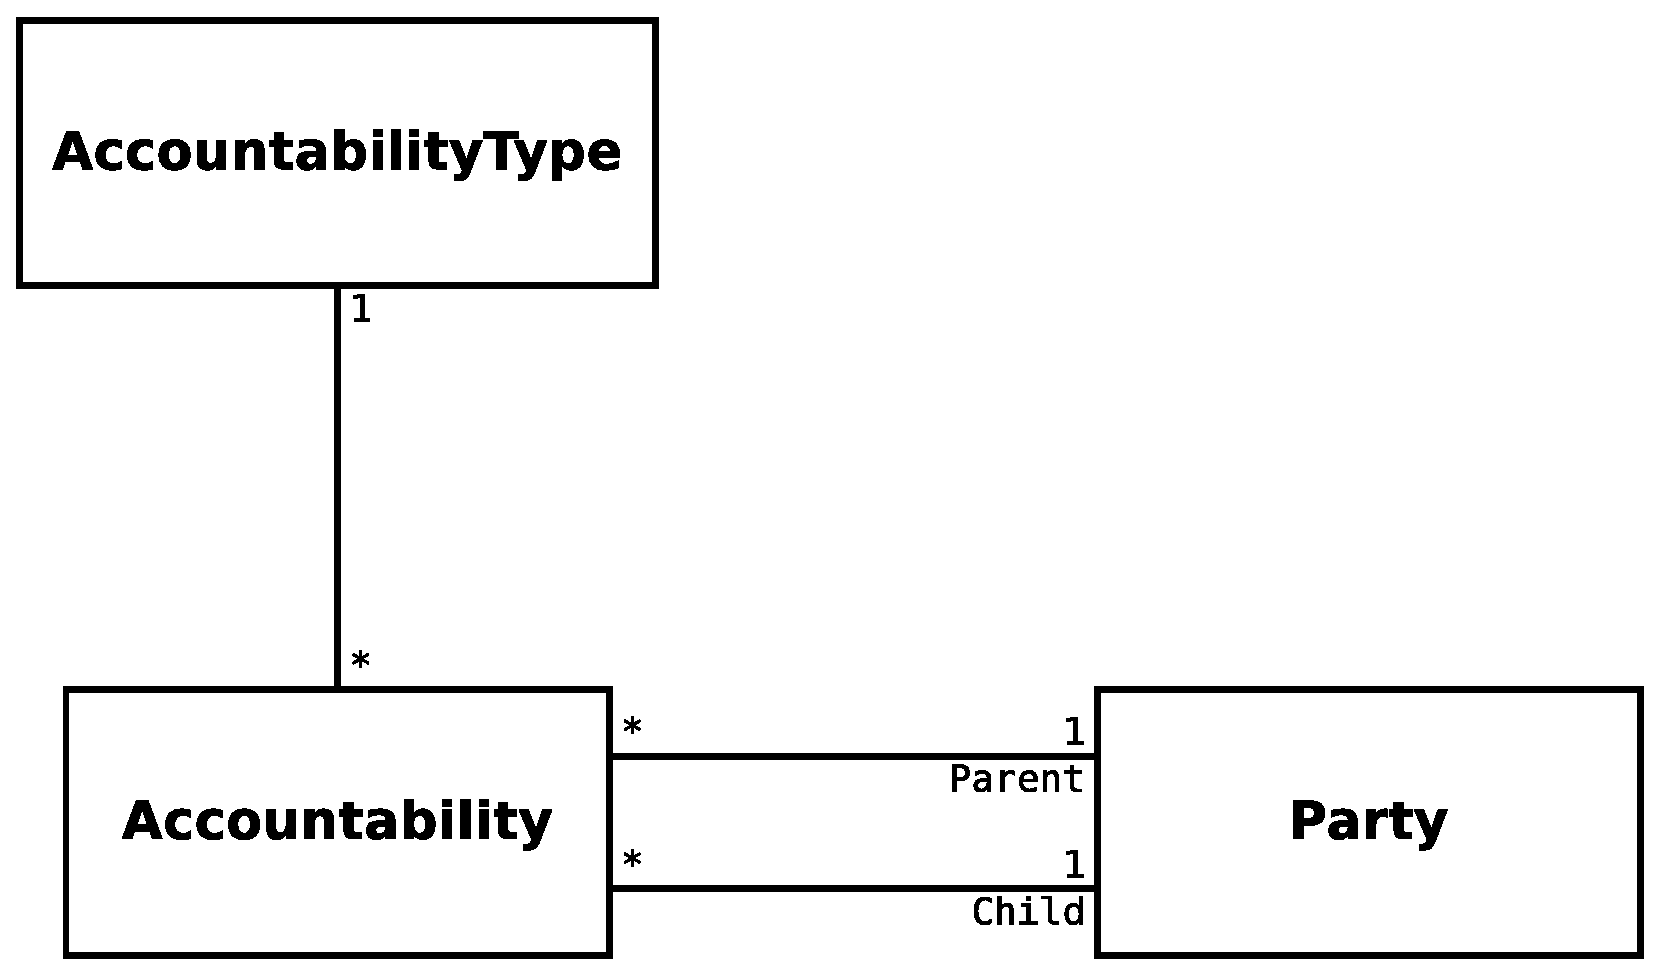
\includegraphics[width=100mm]{accountability}
  \caption{\textsc{Accountability} pattern, adapted from \cite{fowler_accountability}}
  \label{fig:accountability}
\end{figure}

Most OOP languages, however, describe object attributes as either primitive values or references to other objects. Some languages, such as Ruby and Smalltalk, treat everything as an object and do not make any difference between references and primitive values. These concepts can be used to extend the \textsc{Property} pattern, and make it aware of relationships between entities, using attributes such as cardinality, navigability or role~\cite{aom_research_roadmap}.

The revised \textsc{Property} pattern is depicted in Figure \ref{fig:property_revised}:

\begin{figure}[H]
  \centering
  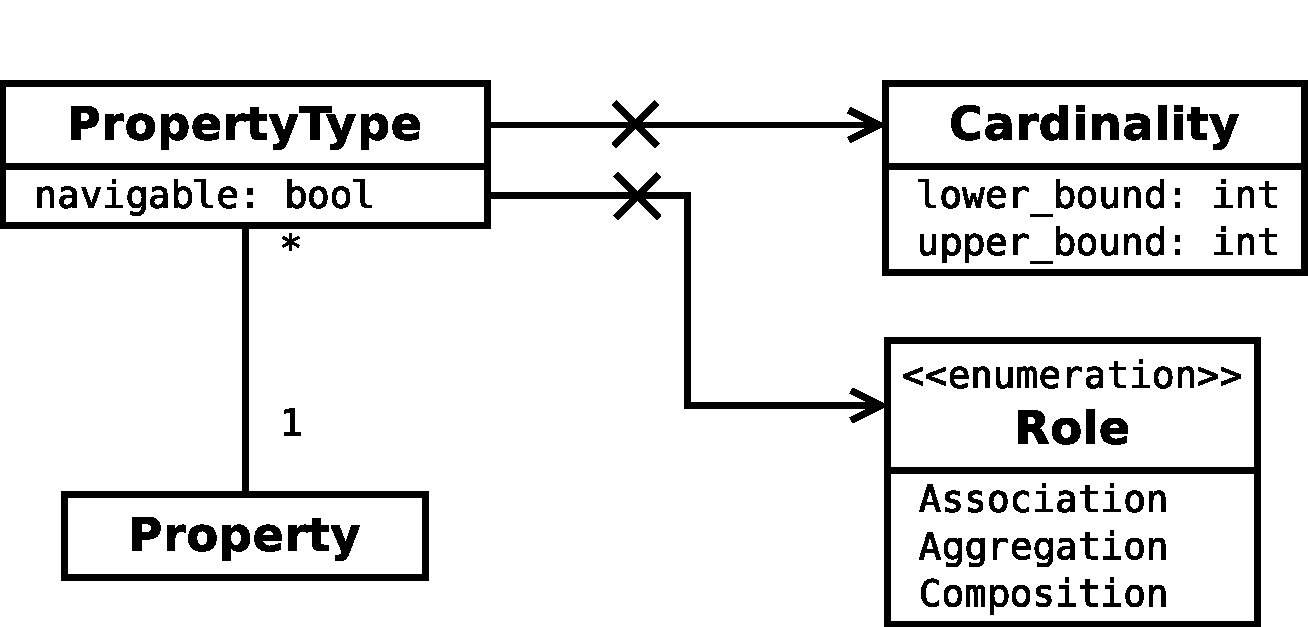
\includegraphics[width=100mm]{property_revised}
  \caption{Revised \textsc{Property} pattern, adapted from \cite{aom_research_roadmap}}
  \label{fig:property_revised}
\end{figure}

\subsection{Pattern Composition}\label{sec:aom_pattern_composition}

By themselves, the design patterns described before do not make up an AOM architecture. Mixing up patterns does not provide any concrete implementation of this kind of architectures, nor it points to what a framework for AOM would look like --- which means that the usual architecture of an AOM is usually the result of composing one or more of the aforementioned patterns in conjunction with other object-oriented patterns. The result of this conjunction can be seen in Fig.~\ref{fig:aom_pattern_composition}

\begin{figure}[H]
  \centering
  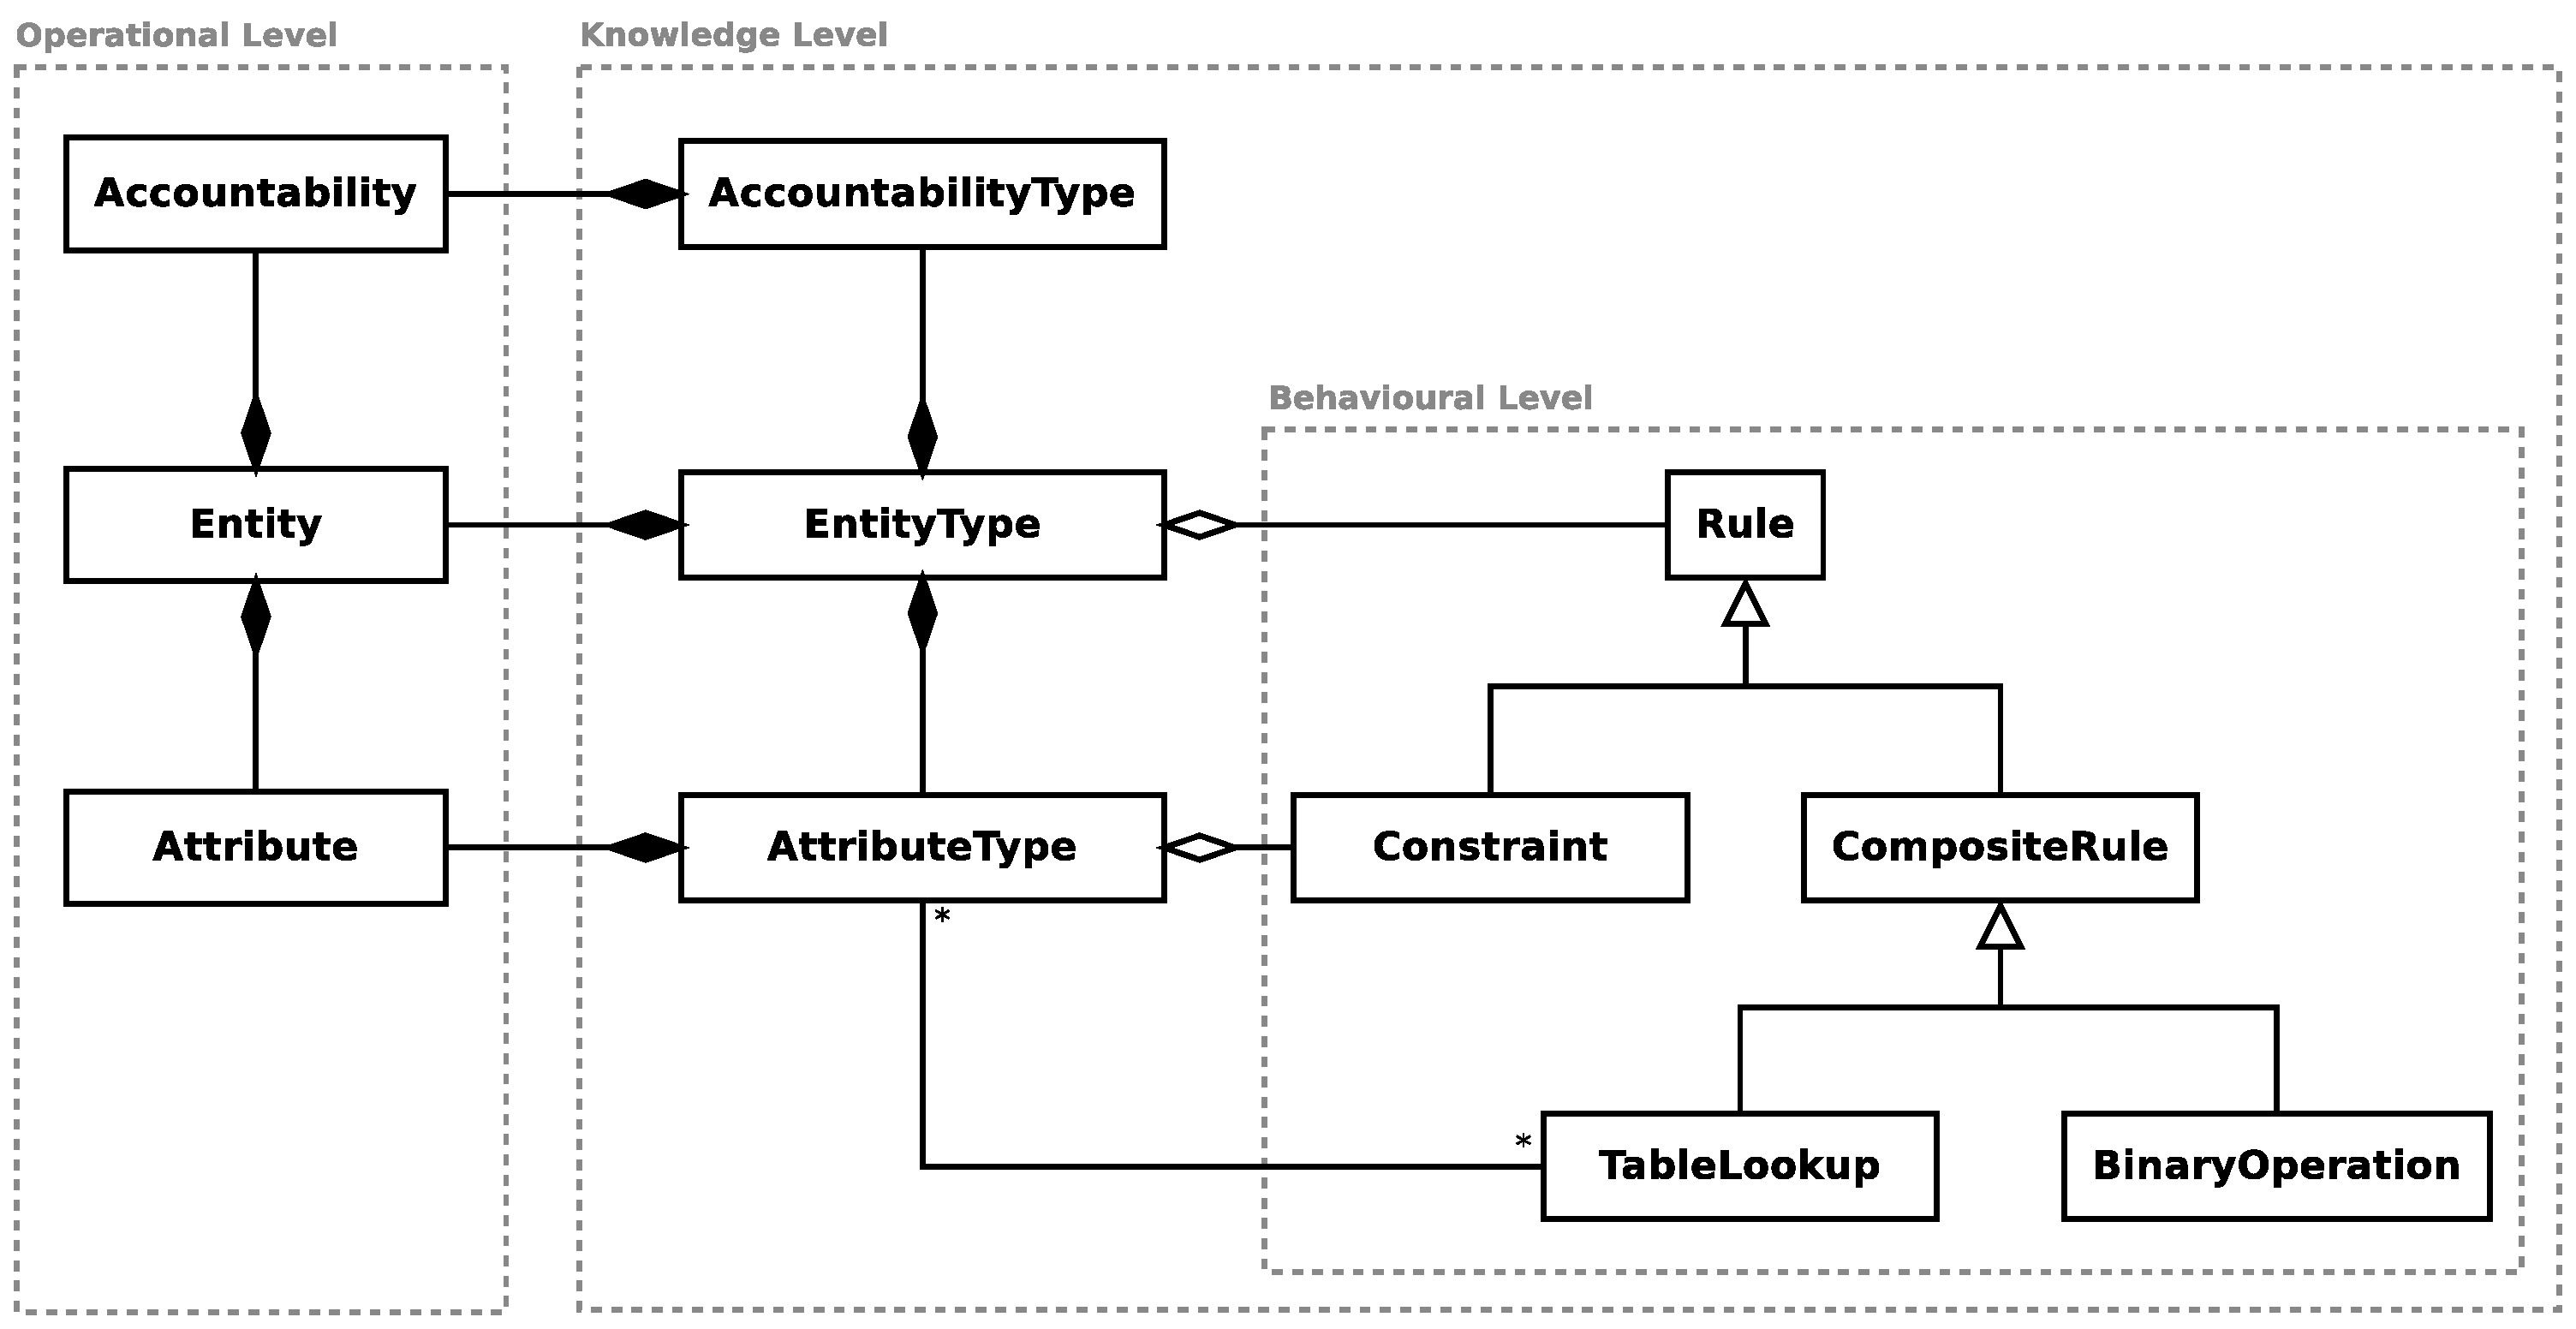
\includegraphics[width=160mm]{aom_pattern_composition}
  \caption{AOM core architecture and design, adapted from \cite{YBJ01}}
  \label{fig:aom_pattern_composition}
\end{figure}

\subsection{AOM GUI Generation}\label{sec:aom_gui_generation}

A system is only as powerful as the interaction with that system allows you to manipulate it --- meaning that a poor interface (be it a GUI or an API or any other kind of interface) does not afford a full-fledged use of the system in question.

Regarding AOM systems, as the system is interpreted and modified in runtime, the GUI must also be automatically built in runtime from the interpretation of the M1 level model. This implies a standardized approach to rendering entities and entity properties, in order to minimize code redundancy and provide a consistent look \& feel. The main problem identified by Welicki et al.\cite{WYW07} was the redundancy that arose from the need to render each type of property, leading to a higher degree of maintenance and potencial UI inconsistency. The solution devised was to create rendering objects responsible for rendering the user interface for each type of property within a given context, creating what is know as the \textsc{Property Renderer} pattern, which enforces a strong separation between domain entities and respective visualization.

However, the separate rendering of single properties is not enough to capture the complexity of an entity. There needs to be a coordination of the various \textsc{Property Renderers} in order to produce a more complex output (be it a UI fragment or a complete interface). The solution is to build view components which coordinate the presentation of several property renderers of an entity to produce different complex UI fragments. Each property renderer is specialized to generate UI code for instances of a property type in a certain context (viewing, editing, different visualization formats, etc). A view component will coordinate several fine-grained renderers and produce more complex UI code for an entity. As such, the same basic concept from \textsc{Property Renderer} can be applied to entities rendering, creating the \textsc{Entity View} pattern~\cite{WYW07}.

\subsection{Oghma}\label{sec:oghma}

Oghma is a reference framework for the development of AOM systems, developed in C\#. It allows the rapid creation of highly variable, dynamic systems. It is currently being developed in the context of the doctoral thesis of Hugo Ferreira. It is a very complete framework able to create, manage and persist AOM systems, from backend to GUI generation, by making extensive use of metaprogramming and metamodeling techniques, by following the general guidelines of the \textsc{Naked Objects} architectural pattern \cite{naked_objects}.

Oghma is thus a concrete implementation of a framework based on the reference architecture to develop AOM-based systems established in~\cite{ferreira_phd_2010}, that balances several design and engineering forces. It supports the creation of models resembling MOF~\cite{mof} and UML~\cite{uml}, and aims at covering the entire cycle of system creation and evolution. As an AOM, it allows the introduction of changes to the system during runtime, thus providing a particular kind of confined end-user development. Fig.~\ref{fig:oghma_core_architecture} show the core architecture for this framework.

It is structured as a collection of \textsc{Layered Component Library} \cite{metaprogramming_metamodeling}, allowing their high-level composition to achieve different functional architectures, e.g. client-server v.s. single-process.

Furthermore, the framework leverages the infrastructure used to support system evolution to provide additional features, such as auditing over the system’s usage, and time-traveling to an arbitrary point along its evolution (i.e. to set the system in a past state).

Oghma includes a set of interchangeable components designed to have an high degree of flexibility, as it was designed to support several types of persistency engines --- be it in memory or a DBMS.

Finally it adds the ability to specify a wide set of behavioural and validation rules by using the \textsc{Interpreter} pattern\cite{gang_of_four}, presenting to the end-user as a  DSL, either through a textual syntax or a graphical interface representative of the rules to be enforced.

\begin{figure}[H]
  \centering
  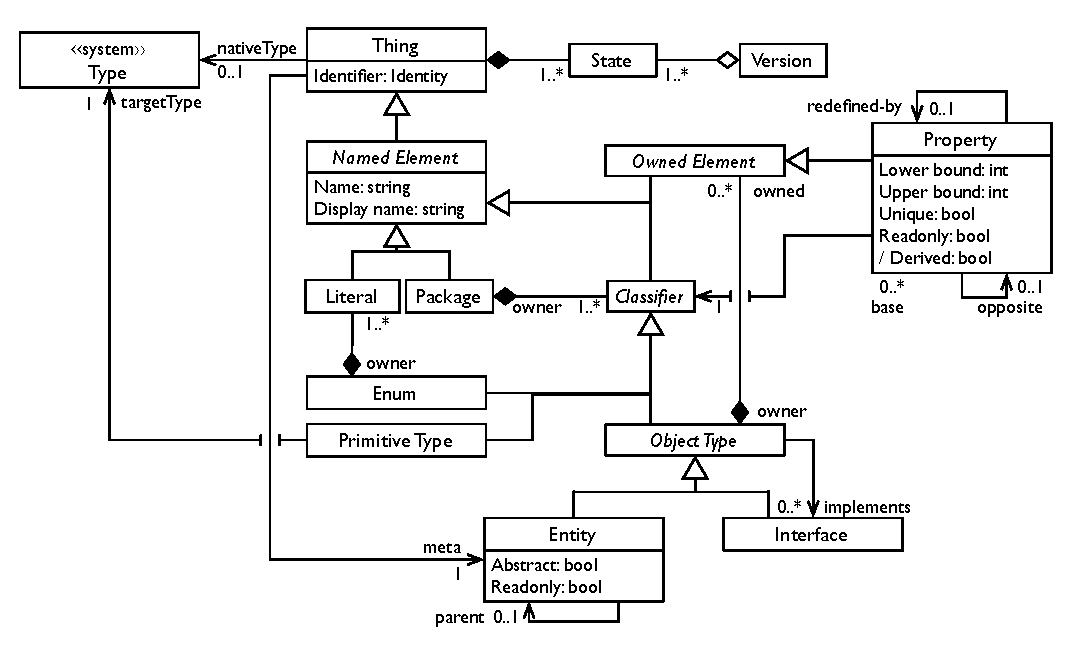
\includegraphics[width=140mm]{oghma_core_architecture}
  \caption{Implementation model of the structural meta-model for the Oghma framework}
  \label{fig:oghma_core_architecture}
\end{figure}

\section{Ruby}\label{sec:ruby}

Ruby is a dynamic, purely object-oriented programming language. It was created by Japanese programmer Yukihiro Matsumoto and it was first released to public in 1995. In its author words, Ruby was created to be a ``a dynamic, open source programming language with a focus on simplicity and productivity. It has an elegant syntax that is natural to read and easy to write''~\cite{ruby}. It was inspired by many different languages such as Lisp, Smalltalk, Perl and Ada, and possesses a series of characteristics that make it extremely attractive~\cite{ruby}.

The Ruby language was designed with a meta-architecture in mind: it allows for changes to class definitions in runtime, constantly adapting to change. It does so by providing open, active class definitions. A common part of the development process when writing a Ruby program is to extend the language by extending the core language classes (such as \verb!String! and \verb!Float!) with custom methods~\cite{metaprogramming_ruby}.

\subsection{Ruby Metaprogramming}\label{sec:ruby_metaprogramming}

Ruby uses metaprogramming techniques extensively --- in fact, metaprogramming is an integral part of some of the language constructs. Take the example from Listing~\ref{fig:ruby_class_metaprogramming}

\begin{lstlisting}[language=ruby, float=htb, label=fig:ruby_class_metaprogramming, caption=Metaprogramming in Ruby classes.]
 class Person
   attr_accessor :name, :age
 end
\end{lstlisting}

The use of the \verb!attr_accessor! declaration is actually a shortcut method for a \emph{getter} and \emph{setter} for the \verb!name! and \verb!age! attributes of the \verb!Person! class. It does so by automatically creating the necessary methods inside a \verb!class_eval! context --- effectively modifying the class definition by evaluating code in runtime. Figure~\ref{fig:ruby_class_metaprogramming_after} represents the code generated internally by the Ruby interpreter when interpreting Listing~\ref{fig:ruby_class_metaprogramming}:

\begin{lstlisting}[language=ruby, float=htb, label=fig:ruby_class_metaprogramming_after, caption=Code generated by Ruby metaprogramming constructs.]
 class Person
   def name=(val)
     @name = val
   end
   def name
     @name
   end
   
   def age=(val)
     @age = val
   end
   def age
     @age
   end
 end
\end{lstlisting}

The usage of the metaprogramming facilities present in Ruby is important in the context of AOM architectures: as a dynamic language, it is able to manipulate and generate code in runtime. This special property of Ruby (and other dynamic languages, such as Python) allows the simplification of many of the patterns described before, especially \textsc{Property} --- by using the capabilities of the language, these patterns are absorbed by the language itself, becoming a normal part of development.

\subsection{Ruby On Rails}\label{sec:ror}

Ruby on Rails is a full-stack Web framework, initially developed by Hansson in 2003, based on the MVC design pattern. As stated by~\cite{rubyonrails}:

\begin{quote}
  ``Ruby on Rails is an open-source that's optimized for programmers happiness and sustainable productivity. It lets you write beautiful code by favoring convention over configuration.''
\end{quote}

In regards to code generation, the Ruby on Rails framework includes a series of mechanisms for system artifacts generation, be it Models, Controllers or even Views. It does so by analyzing the underlying relational database model and deriving the model specifications from the column's type and name. However, RoR does not generate a static model definition, as it deduces the necessary information whenever the system is loaded. Instead, it uses these informations to create an adequate code skeleton for basic CRUD operations in views, greatly accelerating the development process by providing the developers with a basic blueprint of a fully functional system that can be refined and tailored to specific needs~\cite{rails_generators}.
